\section{Discussion} \label{sec:discussion}

We will now describe two experiments evaluating the quality of the \el\
algorithm's output and the efficiency of both of our algorithms, and
we discuss the interface between our algorithms and realization.


%different aspects of
%the performance of our algorithm. First, we will look at its running
%time on randomly generated domain graphs of different sizes. Second,
%we will compare the output of our algorithm to human-generated
%descriptions.



\subsection{Evaluation: Output quality}

To compare the descriptions generated by our algorithm to those humans
produce, we use a corpus of human-generated referring expressions
collected and made available by Jette Viethen and Robert
Dale.\footnote{http://www.ics.mq.edu.au/\~{}jviethen/drawers}  They
asked human subjects to describe one of 16 filing cabinet drawers. The
drawers had different colors and were arranged in a four-by-four grid
(see Fig.~\ref{fig:drawers}). The human subjects used seven
non-relational properties (the drawer's color, its $\mathsf{column}$
and $\mathsf{row}$ number, and whether it is in a $\mathsf{corner}$)
and five relational properties ($\mathsf{above, below, next\ to, left\
  of, right\ of}$). Of the 118 referring expressions, only 15 use
relations.

\begin{figure}
\begin{center}
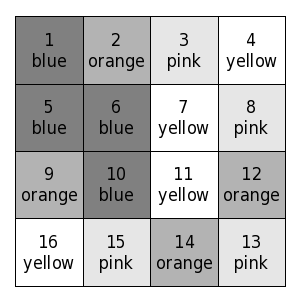
\includegraphics[width=0.25\textwidth]{drawers.png}
\end{center}\vspace*{-3ex}
\caption{A schematic view of the filing cabinets.}\label{fig:drawers}\vspace*{-3ex}
\end{figure}


\newcite{viethen06:_algor_for_gener_refer_expres} describe the data in
more detail and present results of evaluating the Full Brevity
algorithm, the Incremental Algorithm (both by \newcite{Dale1995}), and
the relational algorithm \cite{dale91:_gener_refer_expres_invol_relat}
on this corpus. The Incremental Algorithm is dependent on a predefined
ordering in which properties are added to the description. Viethen and
Dale, therefore, try all possible orderings and evaluate what
percentage of descriptions an algorithm can generate with any of
them. The Full Brevity and the Relational Algorithms choose properties
based on their discriminatory power and only use the orderings as tie
breakers. Viethen and Dale found that the Incremental Algorithm is
capable of generating 98 of the 103 non-relational
descriptions. However, the Dale and Haddock algorithm was unable to
generate even a single one of the human-generated relational
descriptions.

%(using four different orderings to cover all the data). 

\input example-outputs

We replicated Viethen and Dale's experiment for the \el\ algorithm
presented above. In the non-relational case, our results are the same
as theirs for the Incremental Algorithm: the \el\ algorithm generates
98 of the 103 non-relational description.  This is because the two
algorithms perform essentially the same computations if there are no
relations.


To evaluate the relational case, we first removed the
$\mathsf{column}$ and $\mathsf{row}$ predicates from the domain,
because these predicates make it possible to uniquely identify each
drawer with non-relational descriptions, and our algorithm would
always prefer these.  Using three (of 240) different orderings, our
algorithm was able to generate 10 of the 15 human-produced relational
descriptions correctly.  This is shown in more detail in
Fig.~\ref{fig:example_outputs}; notice that four of the 15
descriptions occurred twice in the corpus.  Of the five human-produced
descriptions that the \el\ algorithm cannot generate, two mention
column information, which we excluded from our domain, and three
involve references to sets (\textit{the two blues ones in horizontal
sequence}/\textit{the two yellow drawers}). While our algorithm cannot
reproduce those descriptions, it does generate other, simpler
descriptions for them.








\subsection{Evaluation: Efficiency}

Both the \el\ and the \alc\ algorithms took about 15 milliseconds to
compute distinguishing formulas for all 16 individuals in the Viethen
and Dale dataset.\footnote{Runtimes are meassured on a MacBook Pro
  (Intel Core 2 Duo, 2.16 GHz) running Java 1.6 beta, and we allowed the
  Java VM to warm up, i.e., just-in-time compile all bytecode, before
  taking the measurements.}

In order to get a more comprehensive picture of the algorithms'
efficiency, we ran them on random models with increasing numbers of
individuals.  Each model had random interpretations for ten different
propositional and four relational symbols; each individual had a 10\%
chance to be in the extension of each propositional symbol, and each
pair of individuals had a 10\% chance to be related by a relational
symbol.  The results (averaged over 10 runs for each model size) are
shown in Fig.~\ref{fig:runtimes}.  As the figure shows, the \el\
algorithm takes about 350 ms on average to generate relational REs for
all individuals in the model of size 100, i.e.\ less than 4 ms on
average for each individual.  The \alc\ algorithm is even faster, at
about 140 ms for the model of size 100.  As far as we know, these are
by far the fastest published runtimes for any relational GRE algorithm
in the literature.

Another encouraging aspect of both runtime graphs is that they seem to
be approximated well by quadratic functions.  So although the
worst-case runtime of the \el\ algorithm might be exponential, both
algorithms empirically exhibit (low) polynomial runtime on the inputs
we considered.



\subsection{Interface to realization}
\label{sec:discussion-realization}

%\begin{itemize}
%\item there's a risk to generate a formula that can't be realized,
%  especially for the \alc\ algorithm
%\item everybody except perhaps SPUD has this problem
%\item problem is worse in our case because it is harder to control the
%  order in which atoms and relations are explored
%\item would be interesting for future work to think about how
%  search in the bisim algorithms can be controlled by the realizer
%\end{itemize}

Our GRE algorithms do not guarantee that the formula they compute can
actually be realized in language.  For example, none of the formulas
our algorithms computed in the Viethen and Dale domain contained an
atom that would commonly be realized as a noun; the property
$\mathsf{drawer}$ is never used because it applies to all individuals
in the domain.  This particular problem could easily be worked around
in a post-processing step.  However, another problem arises from the
massive use of negation in the \alc\ algorithm; it will be hard for
any realizer to find a reasonable way of expressing a formula like
$\neg \exists R.(\neg P \sqcap \neg Q)$ as a smooth noun phrase.
Although we agree with \newcite{deemter01:_gener_refer_expres} and
others that the careful use of negation and disjunction can improve
REs, these connectives must not be overused.  Thus we consider the
formulas computed by the \el\ algorithm ``safer'' with respect to
realization.


\begin{figure}[t]
  \centering
  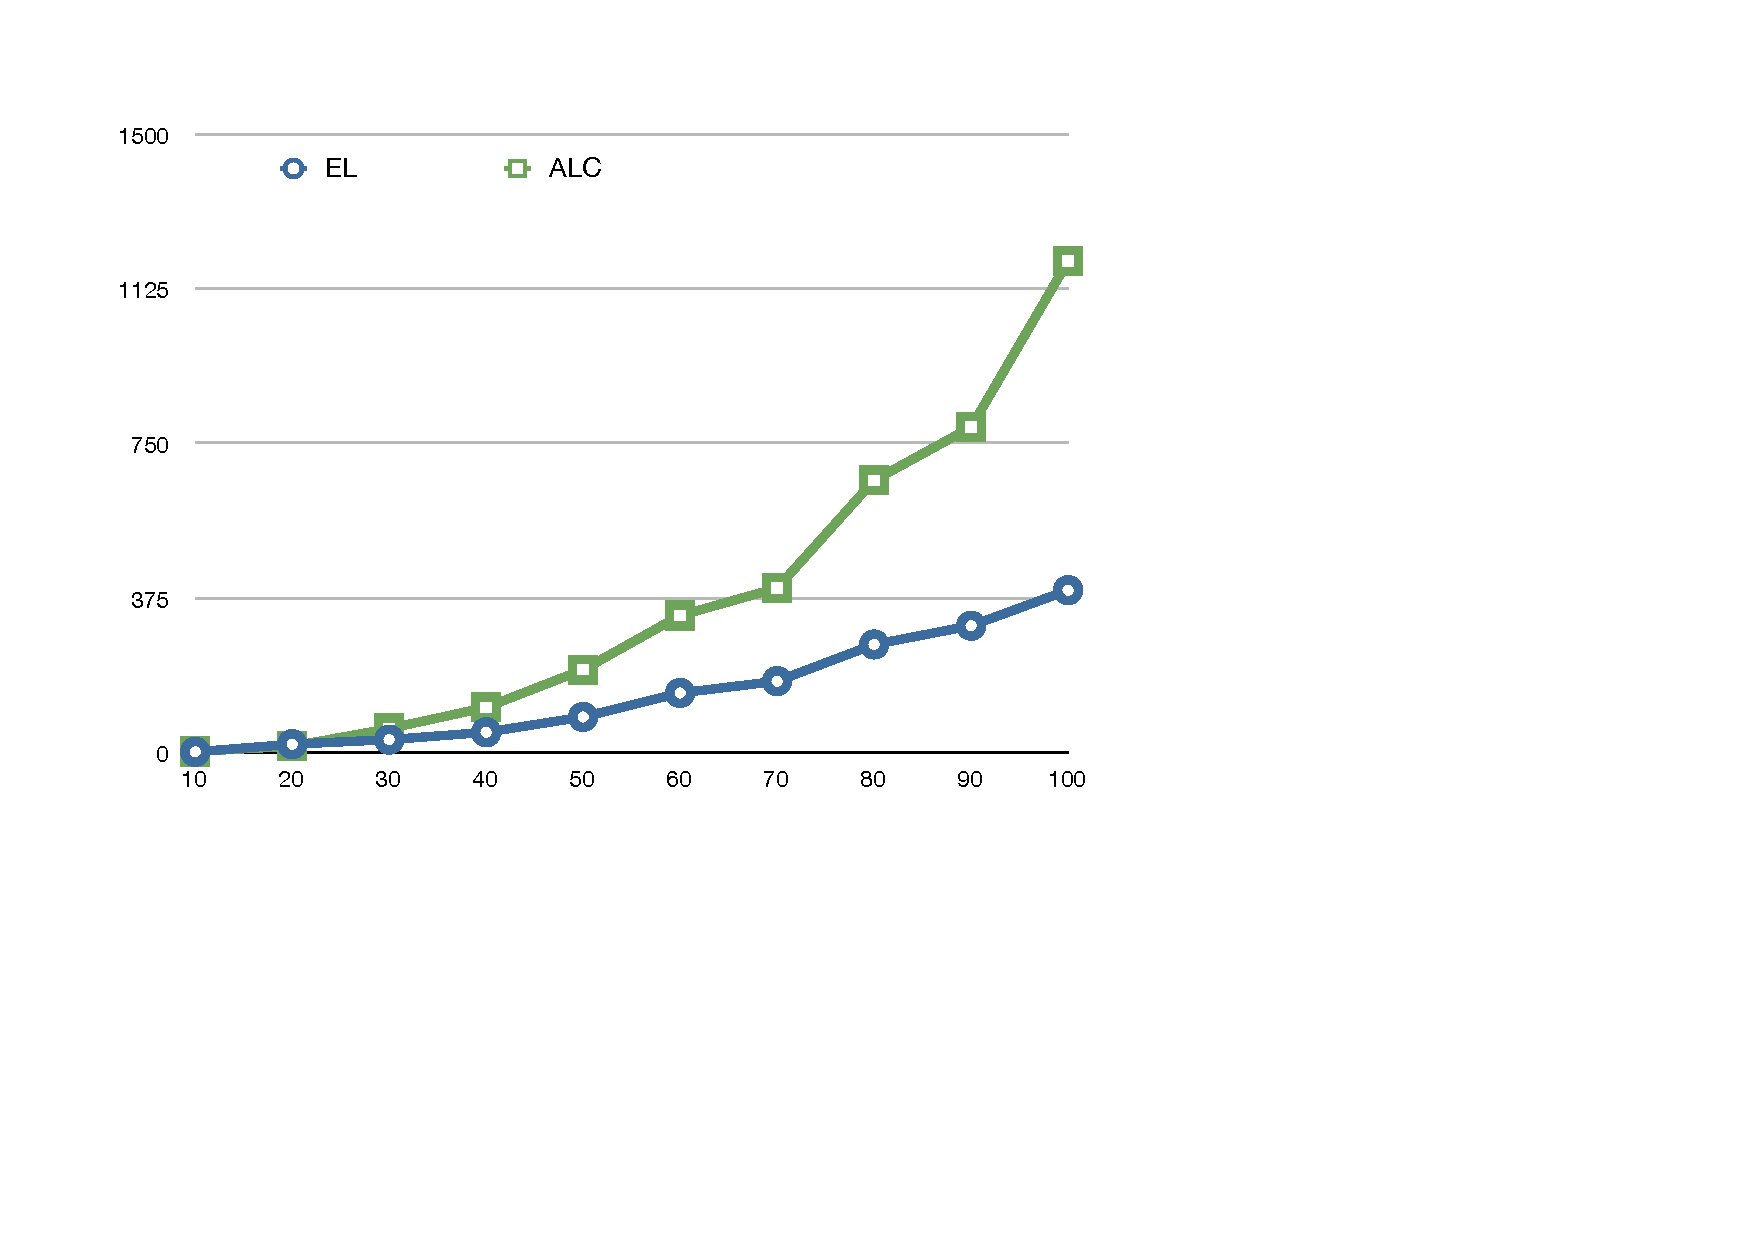
\includegraphics[width=\columnwidth]{runtimes}
  \caption{Average runtimes (in ms) of the two algorithms on random
    models with different numbers of individuals.}%%of different sizes.} 
  \label{fig:runtimes}
\end{figure}

Of course, we share the problem of interfacing GRE and realization
with every other approach that separates these two modules, i.e.\
almost the entire GRE literature (notable exceptions are e.g.\
\newcite{Horacek1997} and SPUD \cite{Stone1998a}).  In principle, we
believe that it is a good idea to handle sentence planning and
realization in a single module; for instance, SPUD can use its
awareness of the syntactic context to generate succinct REs as in
``take the rabbit from the hat''.  We hope that the ideas we have
explored here for efficient and expressive RE generation can
eventually be combined with recent efficient algorithms for integrated
sentence planning and realization, such as in \newcite{KolSto07}.

One problem that arises in our approach specifically is that the
bisimulation classes algorithms derive some measure of efficiency from
their freedom to build formulas without having to respect any
linguistic constraints.  It seems straightforward, for instance, to
extend Krahmer et al.'s \shortcite{Krahmer2003} approach such that it
only considers subgraphs that can actually be realized, because their
algorithm proceeds by a genuine search for uniquely identifying
subgraphs, and will simply take a different branch of the search if
some subgraph is useless.  This would be harder in our case.  Our
algorithms don't search in the same way; if we disallow certain
refinements of a partition, we have to allow the algorithms to
backtrack and thus jeopardize the worst-case polynomial runtime.
Investigating this interplay between efficiency and linguistic
constraints is an interesting avenue for future research.




%%% Local Variables: 
%%% mode: latex
%%% TeX-master: "dl-gre-08"
%%% End: 
